\documentclass{article}

\usepackage{xcolor}
\usepackage{inconsolata}
\usepackage[T1]{fontenc}
\usepackage{pgffor}
\usepackage{graphicx}
\usepackage{fancyhdr}
\usepackage{hyperref}
\usepackage{tcolorbox}
\usepackage[margin=1.2in]{geometry}
\usepackage{biblatex}
\addbibresource{refs.bib}

\hypersetup{
  colorlinks=true,
  linkcolor=blue,
  filecolor=magenta,
  urlcolor=blue,
}

\renewcommand*\familydefault{\ttdefault} %% Only if the base font of the document is to be typewriter style

\newcommand{\topic}[1]{\tcbox[on line,arc=4pt,colframe=white,boxrule=0pt,boxsep=0pt,left=4pt,right=4pt,top=3pt,bottom=2pt,colback=gray!30]{#1}}

% Define a custom command for colored boxes around words
\newcommand{\topics}[1]{%
  \linebreak
  \linebreak
  \foreach \word in {#1} {%
    \topic{\word}%
  }%
  \linebreak
}


\title{Bachelor Ideen}
\author{Max Richter}

\begin{document}
\raggedright
% \pagecolor[rgb]{0.05,0.05,0.05}
% \color{white}
\maketitle
\pagebreak
\section{Node-Based UI's}
Node-Based Interfaces sind eine besondere Unterart der visuellen Programmiersprachen. 
Sie werden häufig in 3D-Software verwendet, um komplexe Szenen zu erstellen. 
Ein Node-System besteht aus Nodes, die miteinander verbunden werden können. 
Jede Node hat eine bestimmte Funktion. Man kann die einzelnen Nodes miteinander verbinden, so das die Ausgabe einer Node als Eingabe für eine andere Node verwendet werden kann.
\linebreak
\linebreak
Dadurch können komplexe Strukturen erstellt werden, die auch für Anfänger leicht zu verstehen sind.
\linebreak
\linebreak
\begin{figure}[h]
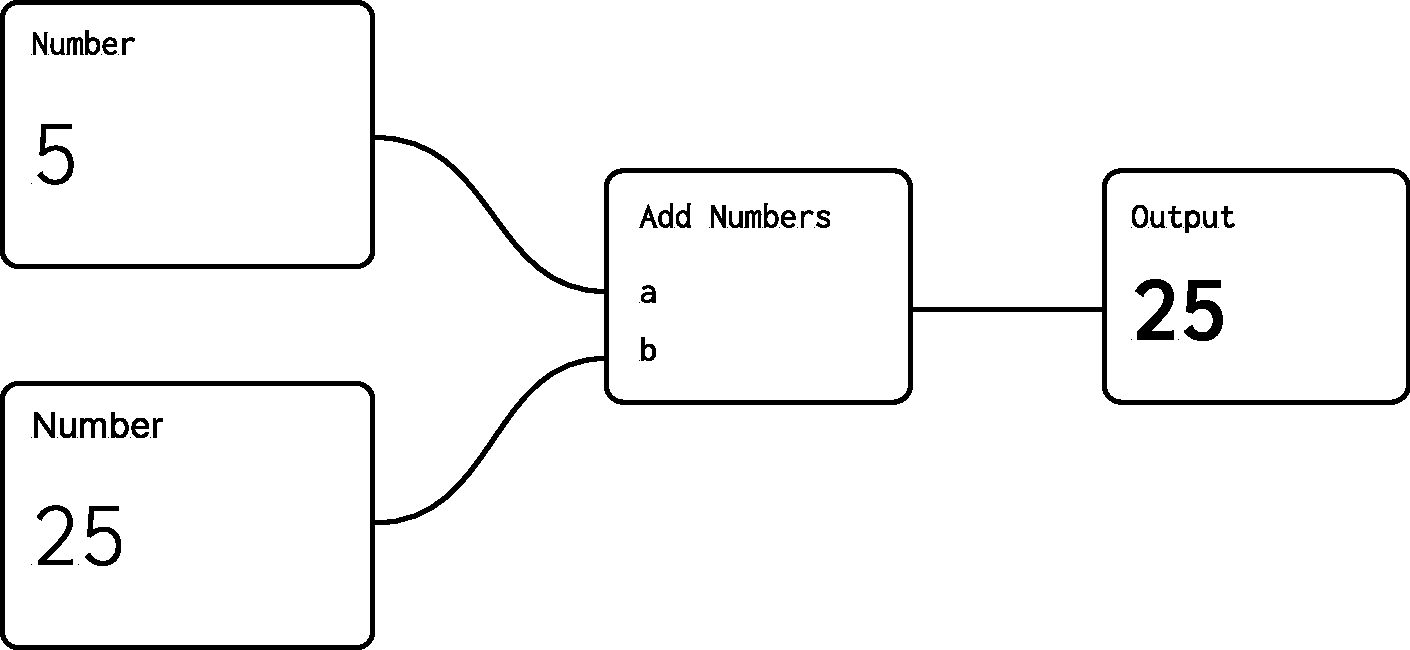
\includegraphics[width=\textwidth]{ideas/nodes.pdf}
\caption{So könnte ein Node-System aussehen}
\end{figure}

Node-based interfaces sind deutlich komplexer als die meisten "klassischen" Interfaces. Dafür bieten sie dem/der Nutzer*in deutlich mehr Freiheit und Möglichkeiten. 
\linebreak

Sie sind ein wunderbarer Mittelpunkt zwischen der Komplexität und großer Freiheit einer Programmiersprache und der Einfachheit eines klassischen Interfaces.

Vorallem das es Menschen die nicht Programmieren können ermöglicht, komplexe Strukturen zu erstellen finde ich sehr spannend.

\pagebreak


\subsection{Beispiele für Nodesysteme}

Die Opensource 3D Software Blender benuzt ein Node-System für die Erstellung von Materialien und Texturen. In neueren Versionen sogar für die Erstellung von 3D Objekten und Animationen.

\begin{figure}[h]
\centering
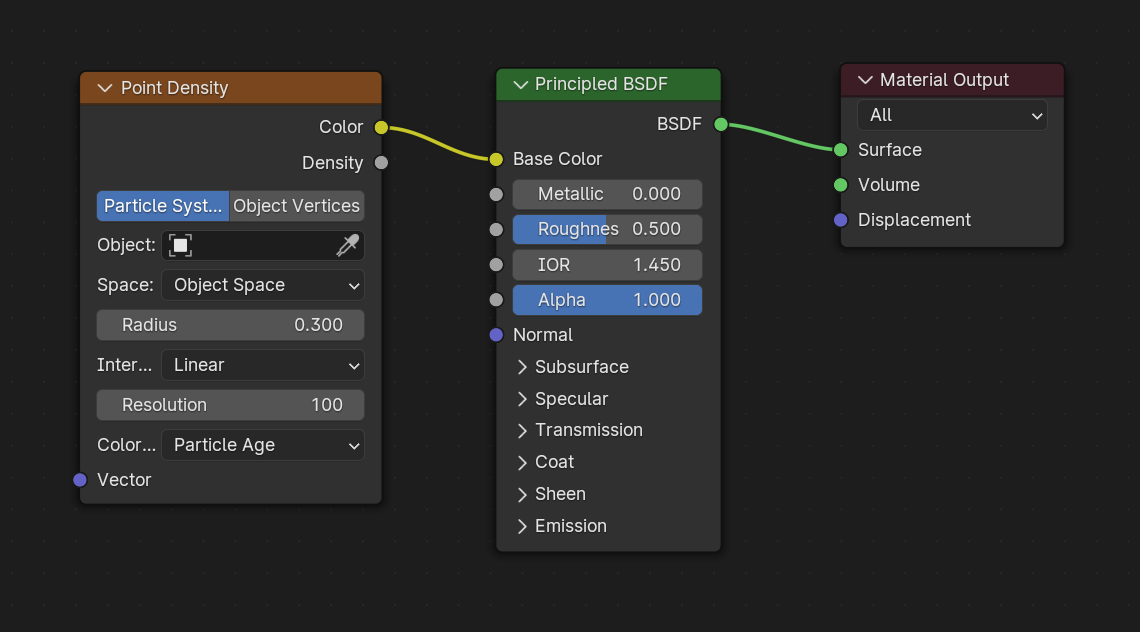
\includegraphics[width=0.8\textwidth]{ideas/blender-shader.png}
\caption{Shader System der 3D-Software Blender}
\end{figure}

Die 3D-Software Houdini ist komplett auf Node-Systeme aufgebaut. Sogar die Benutzeroberfläche ist ein Node-System. Houdini wird in Hollywood für die Erstellung von Spezialeffekten verwendet.

\begin{figure}[!ht]
\centering
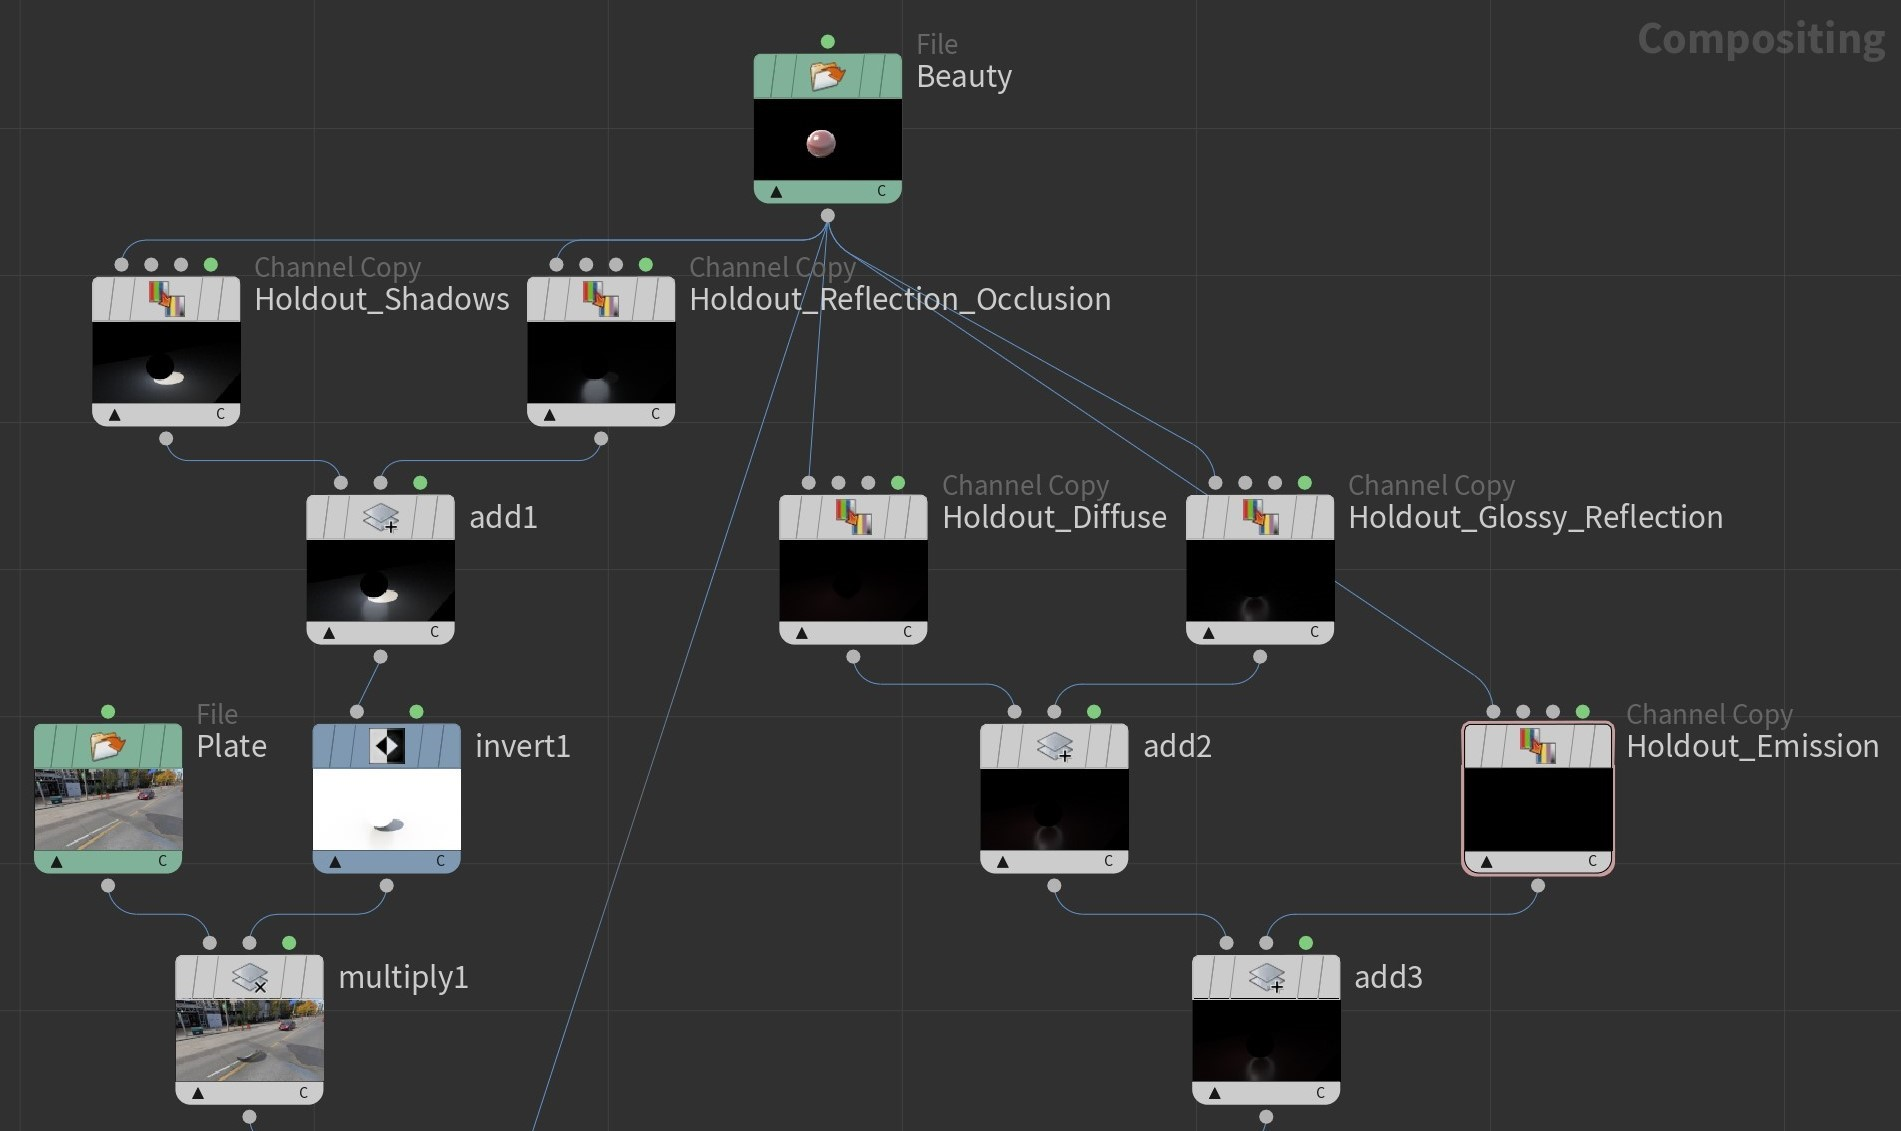
\includegraphics[width=0.8\textwidth]{ideas/houdini-nodes.jpg}
\caption{Node-System der 3D-Software Houdini}
\end{figure}

\subsection{Mögliche Themen zu Node-Based UI's}

\subsubsection{Node-Based Interfaces für Menschen ohne Programmierkenntnisse}
Wie kann man Node-Based Interfaces einsetzen um komplexe Systeme zu erstellen, ohne das der/die Nutzer*in programmieren können muss?
\linebreak
\linebreak
Und wie kann man Menschen den Umgamg mit Node-Systemen beibringen die noch nie damit gearbeitet haben? Welche Konzepte und Ideen gibt es, um Menschen den Einstieg zu erleichtern?
\topics{Didaktik, Lernkonzepte, UIDesign}

\subsubsection{Serialisierung von Node-Systemen}
Wie kann ich die Struktur eines Nodesystems so designen, dass es einfach zu serialisieren ist?
\topics{Linealisierung, Baumstrukturen, Graphen}

\subsubsection{Wie führt man so ein Node-System aus?}
Es gibt viele komplexe Fragestellungen, die aus dem Design eines Nodesystems resultieren. Ist es möglich Schleifen dazustellen und wie führt man diese effizient aus?
\linebreak
\linebreak
Wie designt man das Node-System so, das es effizient ausgeführt werden kann?
\topics{Algorithmen, Graphen, Linealisierung}

\subsubsection{Designen eines erweiterbaren Node-Systems}
Wenn man darüber nachdenkt, sind einzelne Nodes nur Funktionen, sie erhälten Parameter und geben einen Wert zurück. 
\linebreak
Ich fände es sehr spannend, ob es möglich ist etwas zu designen, was eine Sammlung von Funktionen in Nodes verwandelt. 
\topics{Funktionen, Erweiterbarkeit, Modularität, Parser}
\pagebreak

\section{Structured Note-Taking}

Während meines Ausslandsemesters in Spanien habe ich mich ausversehen in eine Vorlesung für Elektrotechnik eingeschrieben, die mich damals komplett überfordert hat.
\linebreak
\linebreak
Ich musste komplette Grundlagen nachholen. Dafür habe ich angefangen zu recherchieren wie man effizient lernt und bin auf das Thema Structured Note-Taking gestoßen.
\linebreak
\linebreak
Es gibt viele verschiedene Arten von Structured Note-Taking, aber das Grundprinzip ist immer das gleiche. Man schreibt alle seine Notizen in einer bestimmten Struktur und kann die einzelnen Notizen miteinander verknüpfen.
\linebreak
Es ist etwa wie ein kleines privates Wikipedia vorstellen, wo es zum Beispiel ein Artikel zu dem Thema Ohmsches Gesetz gibt und ein Artikel für die nächste Klausur und diese können miteinander verknüpft werden.
\linebreak
\linebreak
Vorallem die Idee alle Bereiche seines Lebens in Notizen niederzuschreiben und miteinander zu verknüpfen finde ich sehr spannend. Diese Unterart des Structured Note-Takings wird oft \textit{Second Brain} genannt.
\linebreak
Dazu kommt noch das man seine Notizen in leicht zu speichernden Formaten wie Markdown oder TXT speichern kann und sie so leicht durchsuchbar, veränderbar, offen, future-proof und versionierbar sind.
\pagebreak

\subsection{Mögliche Themen zu Structured Note-Taking}

\subsubsection{Vergleich verschiedener Structured Note-Taking Methoden}
Leider ist das Thema Structured Note-Taking gefundenes Fressen für Online Effizienz-Gurus. Und vielen von diesen Gurus vermarkten ihre eigenen Methoden mit dazugehörigen Workshops und Kursen.
\linebreak
Ich bin der Meinung das die Struktur der eigenen Notizen im bestenfall organisch mit den Anforderungen wächst, fände es aber dennoch spannend eine Übersicht und Analyse der verschiedenen Methoden zu erstellen.
\topics{PARA, Zettelkasten, Luhmann, Notizen}

\subsubsection{Vergleich verschiedener Tools für Structured Note-Taking}
Es gibt viele verschiedene Tools für Structured Note-Taking. Ich fände es spannend diese Tools zu analysieren und zu vergleichen. 
\topics{Usability, Design, Ethics, Data-Autonomy}

\subsubsection{Effektive Nutzung von strukturierten Notizen im beruflichen Umfeld}
Ich glaube, Struktured Note-Taking kann für viele Bereiche einen Vorteil bringen, vorallem die Offenheit der Formate und die Möglichkeit die Notizen miteinander zu verknüpfen könnte im beruflichen Umfeld sehr hilfreich sein.
\topics{Effizienz, Notizen, Second Brain}

\subsubsection{Technologische Innovationen im Bereich strukturiertes Notieren}
Ich habe in den letzten zwei Jahren viele unterschiedliche Technologien benutzt, um mit meinen Notizen zu arbeiten. Darunter gab es einige sehr spannende Ansätze die man analysieren könnte.
\linebreak
Aktuell arbeite ich zum Beispiel an einem Hobbyprojekt was meine Notizen in eine Grafen-Datenbank speichert und sie so leicht durchsuchbar macht.
\linebreak
\linebreak
Aber auch die Möglichkeit die persönlichen Notizen in eine Vektordatenbank zu übertragen, und dann mit LLMs mit seinen Notizen zu interagieren finde ich sehr spannend.
\topics{Graphen, Datenbanken, LLMs, Ethics}

\end{document}
